\documentclass[conference]{IEEEtran}
\IEEEoverridecommandlockouts
\usepackage{cite}
\usepackage{amsmath,amssymb}
\usepackage{graphicx}
\usepackage{booktabs}
\usepackage{array}
\usepackage[hyphens]{xurl}
\usepackage{xcolor}
\usepackage[T1]{fontenc}
\usepackage{textcomp}
\renewcommand{\arraystretch}{1.08}

\begin{document}

\title{AI-Based Detection of Phishing, Vishing, and Smishing Attacks: A Multi-Channel Robustness and Attribution Analysis}

\author{
\IEEEauthorblockN{Harshit Kumar}
\IEEEauthorblockA{\textit{Dept. of Information Science \& Engineering}\\
\textit{BMS Institute of Technology \& Management}\\
Bengaluru, India\\
1BY23IS080}
\and
\IEEEauthorblockN{Mohak Kukal}
\IEEEauthorblockA{\textit{Dept. of Information Science \& Engineering}\\
\textit{BMS Institute of Technology \& Management}\\
Bengaluru, India\\
1BY23IS118}
\and
\IEEEauthorblockN{Manish Kumar}
\IEEEauthorblockA{\textit{Dept. of Information Science \& Engineering}\\
\textit{BMS Institute of Technology \& Management}\\
Bengaluru, India\\
1BY23IS107}
\and
\IEEEauthorblockN{Diwakar Kumar}
\IEEEauthorblockA{\textit{Dept. of Information Science \& Engineering}\\
\textit{BMS Institute of Technology \& Management}\\
Bengaluru, India\\
1BY23IS069}
\and
\IEEEauthorblockN{Dr. Shanthi D L}
\IEEEauthorblockA{\textit{Associate Professor, Dept. of ISE}\\
\textit{BMS Institute of Technology \& Management}\\
Bengaluru, India\\
shanthidl@bmsit.in}
}

\maketitle

% =====================================================================
\begin{abstract}
Scams now move between email, SMS and phone calls, yet most detectors cover one
channel and report accuracy on random splits of a single benchmark. We present a
working three-channel system (web dashboard, Gmail integration and an Android app)
that scores each message with a small channel-specific model, adds a per-sender
behaviour profile, and fuses both into one explainable verdict. Every number is
measured on data the model never trained on: held-out template groups, later
time periods, unseen corpora, an unseen person's mailbox and unseen scam-call
channels, with pass/fail rules fixed before scoring. A character n-gram model
scores SMS at macro-F1 0.980 in-source but 0.859 on a held-out corpus, where
smishing recall falls to 0.786. A DistilBERT email model reaches phishing
precision/recall 0.990/0.986 on a later-in-time split and 0.916/0.862 on
2025--26 mail. A link model that sees only the domain reaches ROC-AUC 0.920 but
PR-AUC only 0.585 at a 1.2\% base rate. Sender behaviour lifts spam recall on a
2008 mail stream from 0.611 to 0.912, at the cost of sending 8.5\% of cleared
legitimate mail to the SUSPICIOUS band. On calls, a content layer catches 96.2\%
of scam calls from seven unseen channels while flagging 0.3\% of held-out bank calls; a
wav2vec2 spoof detector catches 85.8\% of voices from 41 unseen synthesis tools,
but at a measured cost on laboratory benchmarks. Finally, we document thirteen
cases in which a public corpus encoded its own collection method, each of which
produced a convincing but false result.
\end{abstract}

\begin{IEEEkeywords}
Phishing, smishing, vishing, social engineering, behavioural profiling,
score fusion, audio anti-spoofing, dataset artifacts, explainable AI.
\end{IEEEkeywords}

% =====================================================================
\section{Introduction}

A modern scam rarely stays in one channel: a phishing mail is followed by a
``verification'' SMS and then by a call from someone claiming to be the bank.
Defences remain siloed. Mail filters do not see SMS, carrier filters do not see
mail content, and calls are judged, at best, by caller-ID reputation. Academic
work mirrors this split, and much of it reports accuracy from random $k$-fold
splits of one benchmark. Scam corpora are full of templates that differ only in a
name or an amount, so a random split puts near-twins on both sides and the score
measures memorisation~\cite{arp2022dos,kapoor2023leakage}.

This paper describes a deployed, end-to-end system built to be tested the hard
way. Its thesis is simple: \emph{content changes with every campaign; the
behaviour of the sender changes far less}. The contributions are:
\begin{enumerate}
\item \textbf{One verdict across three channels.} Small channel models
  (character n-gram SMS model, DistilBERT for mail, a domain-only link model,
  a speech pipeline and a synthetic-voice detector) feed a shared behaviour
  engine and an adaptive fusion rule with explicit abstention (Section~\ref{sec:arch}).
\item \textbf{Leakage-free evaluation with pre-registered rules.} No number in
  this paper comes from a random split; every pass/fail condition was written
  down before the test set was scored (Section~\ref{sec:data}).
\item \textbf{Baselines, ablations, confidence intervals and cost} for every
  channel, including the results that are weak (Section~\ref{sec:results}).
\item \textbf{A catalogue of thirteen corpus artifacts}: features that
  identified the dataset rather than the scam, each found by an ablation or an
  outside test and each worth a convincing false result (Section~\ref{sec:artifacts}).
\item \textbf{Privacy by construction}: SMS is scored entirely on the phone,
  and the app has no network access at all (Section~\ref{sec:ethics}).
\end{enumerate}

% =====================================================================
\section{Related Work}

\textit{Email.} Transformer encoders outperform bag-of-words models on phishing
mail~\cite{uddin2024explainable}, but no single architecture wins across
datasets~\cite{altwaijry2024advancing,alhuzali2025indepth}, and recent work adds
LIME/SHAP explanations~\cite{roshinta2026temporal,calzarossa2024explainable}
and adversarial robustness~\cite{sup2025explainable,kulkarni2024ml2llm}.
Benavides-Astudillo et al.~\cite{benavides2023phishing} combine NLP features with a
BiGRU; a recent survey~\cite{ahmad2025spectrum} notes that most results come from
a few public corpora. \textit{SMS.} BERT~\cite{jain2025smishing},
CNN-LSTM~\cite{mehmood2024smishing} and multi-class deep
models~\cite{boulahaia2025multiclass} report high accuracy, but on static random
partitions. \textit{URLs.} Boosted trees with TreeSHAP are a common
choice~\cite{uddin2025boosting}; isolation forests have been applied to
phishing and traffic anomalies~\cite{lestari2025isolation,chua2024isolation}.
\textit{Voice.} Xing et al.~\cite{xing2020fraudcall} classify call-detail
records; Hong et al.~\cite{hong2023scamcalls} classify ASR transcripts;
Triantafyllopoulos et al.~\cite{triantafyllopoulos2025vishing} argue that
persuasion is the dominant spoken signal; Sim and Kim~\cite{sim2025slm} fine-tune
small language models on transcripts; and Naidoo and
Mhlongo~\cite{naidoo2024smishvish} treat smishing and vishing together with
classical models. Synthetic-voice detection is a separate line:
RawNet2~\cite{tak2021rawnet2}, AASIST~\cite{jung2022aasist} and
self-supervised front ends~\cite{tak2022ssl}, evaluated on the ASVspoof
series~\cite{wang2020asvspoof2019,liu2023asvspoof2021,wang2024asvspoof5} and on
real-world deepfakes~\cite{muller2022itw}, where performance drops sharply.
Table~\ref{tab:related} summarises the gap: no prior system joins the three
channels, and none fuses content with sender behaviour.

\begin{table}[t]
\caption{Representative prior work}
\label{tab:related}
\centering\footnotesize
\setlength{\tabcolsep}{3pt}
\begin{tabular}{@{}p{2.25cm}p{0.95cm}p{1.75cm}p{2.6cm}@{}}
\toprule
Work & Channel & Method & Main limitation \\
\midrule
Xing~\cite{xing2020fraudcall} 2020 & Voice & CDR deep net & Metadata only, no content \\
Benavides~\cite{benavides2023phishing} 2023 & Email & NLP + BiGRU & One channel \\
Hong~\cite{hong2023scamcalls} 2023 & Voice & ASR + LSTM & No synthetic-voice check \\
Altwaijry~\cite{altwaijry2024advancing} 2024 & Email & CNN / BiGRU & One channel, random split \\
Mehmood~\cite{mehmood2024smishing} 2024 & SMS & CNN-LSTM & Static random split \\
Uddin~\cite{uddin2024explainable} 2024 & Email & Transformer & No sender behaviour \\
Jain~\cite{jain2025smishing} 2025 & SMS & BERT & No behaviour, no OOD test \\
Sim~\cite{sim2025slm} 2025 & Voice & Small LM & Text only, no audio \\
Triantafyllopoulos~\cite{triantafyllopoulos2025vishing} 2025 & Voice & Survey & No benchmark \\
\midrule
\textbf{This work} & All 3 & Models + behaviour + fusion & --- \\
\bottomrule
\end{tabular}
\end{table}

% =====================================================================
\section{Data and Evaluation Protocol}\label{sec:data}

\subsection{Datasets}
Table~\ref{tab:data} lists every corpus and what it is used for. Three
sources are private (two team members' mailboxes and one SMS inbox); they
are used only with the owners' consent, never published, and no message text
appears in any log or in this paper.

\begin{table}[t]
\caption{Datasets and their role (Tr = train, Te = held-out test)}
\label{tab:data}
\centering\footnotesize
\setlength{\tabcolsep}{2.5pt}
\begin{tabular}{@{}p{3.65cm}p{0.6cm}p{3.6cm}@{}}
\toprule
Corpus & Role & Notes \\
\midrule
\multicolumn{3}{@{}l}{\textit{SMS (3 classes: ham / spam / smishing)}}\\
UCI SMS Spam~\cite{almeida2011sms}, a rebalanced 10,191-row redistribution of~\cite{mishra2022sms}, Indian fraud SMS, 750 authored Indian promotional SMS (synthetic), one Indian inbox (1,436 rows) & Tr/Te & 17,307 train (with obfuscated twins), 2,596 held-out template groups \\
Mishra--Soni 5,971 release~\cite{mishra2022sms} & Te & 1,780 rows not in the 10,191 file (exact-text dedup) \\
\midrule
\multicolumn{3}{@{}l}{\textit{Email (ham / spam / phishing)}}\\
CEAS-08, Nazario, Nigerian Fraud~\cite{alsubaiey2024dataset} & Tr/Te & CEAS 1--7 Aug vs 8 Aug 2008; phishing split by year inside each corpus \\
Enron, Ling, SpamAssassin~\cite{alsubaiey2024dataset} & Te & 38,407 mails, never trained on \\
phishing\_pot~\cite{phishingpot} + 2 private mailboxes & Tr/Te & $\le$2024 train, 2025--26 test (8,725) \\
CMU Enron~\cite{klimt2004enron}, Enron-Spam~\cite{metsis2006enronspam} & Tr/Te & 1,500 colleague mails; Enron-Spam's 6 boxes held out \\
Third person's mailbox & Te & 791 ham, held out by person \\
\midrule
\multicolumn{3}{@{}l}{\textit{Links}}\\
PhiUSIIL~\cite{prasad2024phiusiil} & Tr & 235,795 URLs, host string only \\
OpenPhish~\cite{openphish} + Tranco~\cite{lepochat2019tranco} & Te & 600 live phishing + 50,000 top sites \\
\midrule
\multicolumn{3}{@{}l}{\textit{Voice content}}\\
FTC robocalls; scam-baiting calls from the channels of~\cite{bhupendra2023scambait} & Tr & 1,353 robocalls; 465 calls, 2 channels held out for model selection \\
HarperValleyBank~\cite{wu2020harpervalley} & Tr/Te & 1,446 bank calls, split in halves A/B \\
Scam-baiting calls, 7 further channels & Te & 105 calls, never seen in training\\
27 recorded two-party calls & Te & 12 scam / 15 legitimate, public recordings \\
\midrule
\multicolumn{3}{@{}l}{\textit{Synthetic voice}}\\
ASVspoof 2019/5~\cite{wang2020asvspoof2019,wang2024asvspoof5}, MLAAD~\cite{muller2024mlaad}, real speech (incl.\ phone calls) & Tr & MLAAD tools split by family \\
ASVspoof 2021 LA~\cite{liu2023asvspoof2021}, In-the-Wild~\cite{muller2022itw}, 41 unseen MLAAD tools, Edge-TTS & Te & 400 per codec $\times$ label for ASV21/ASV5 \\
\bottomrule
\end{tabular}
\end{table}

\subsection{Splits and pre-registered rules}
No $k$-fold cross-validation is used anywhere. SMS is split by \emph{template
group} (the first six words of each Indian message, since 3,200 rows come from
about 1,400 templates; a random split gives a TF-IDF baseline F1 0.99). Email is
split by \emph{time} inside each corpus and, for personal mail, by
\emph{person}. Links are trained on one source (PhiUSIIL) and tested on a
different, live one. Voice is split by \emph{YouTube channel} and by
\emph{corpus}. Before any model was promoted, its pass/fail conditions (e.g.\
``real voices flagged no more than 2 points above the current model'') were
written into the experiment script before the test set was scored; Section~\ref{sec:results}
reports when a model failed one and why it shipped anyway.

\subsection{Setup}
All training ran on one laptop (Intel 13th-generation CPU, 20 threads, 16\,GB RAM, NVIDIA
RTX 4060 Laptop GPU, 8\,GB). Split and sampling seeds are fixed at 0. SMS: \texttt{char\_wb} 3--5-gram TF-IDF
(sublinear) and logistic regression, $C{=}10$. Email: \texttt{distilbert-base-uncased}~\cite{sanh2019distilbert},
256 tokens, 2 epochs, batch 16, AdamW at $3{\times}10^{-5}$, auxiliary
persuasion loss weight 0.3. Links: XGBoost~\cite{chen2016xgboost}, 400 trees,
depth 6, learning rate 0.1, 15 domain-lexical features. Voice: Whisper
small~\cite{radford2023whisper} (faster-whisper, fp16), act model
\texttt{distilbert-base-uncased}, 256 tokens, 3 epochs. Spoof: frozen
wav2vec2 XLS-R 300M~\cite{babu2022xlsr}, layer 20, mean+std pooling, 4\,s crop,
logistic-regression head. Classical models use scikit-learn~\cite{pedregosa2011sklearn}.
Confidence intervals are percentile bootstrap (1,000 resamples)~\cite{efron1993bootstrap}
or Wilson intervals for proportions~\cite{wilson1927}.

% =====================================================================
\section{System Architecture}\label{sec:arch}

\begin{figure*}[t]
\centering
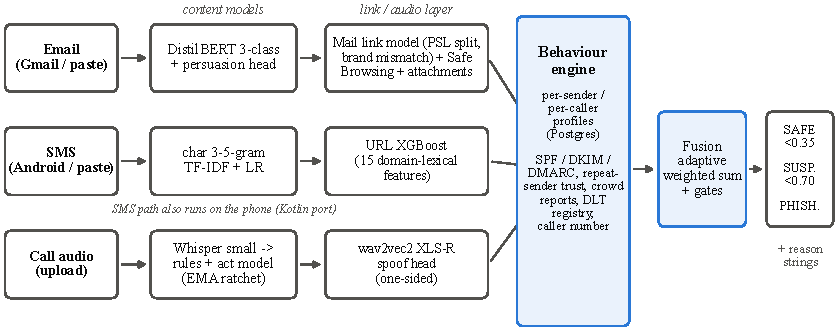
\includegraphics[width=\textwidth]{figs/arch.pdf}
\caption{System overview. Each channel has a content model and a link or audio
layer; all three share the behaviour engine and the fusion rule. The SMS path
also runs fully on the Android phone. A channel with no output abstains and its
weight is redistributed.}
\label{fig:arch}
\end{figure*}

Fig.~\ref{fig:arch} shows the pipeline. A FastAPI service runs the models for the
web dashboard and Gmail; a Next.js dashboard owns the database, sign-in, phone
pairing and Gmail polling; and an Android app scores SMS on the phone with Kotlin
ports of the Python models.

\subsection{Channel models}
\textit{SMS.} SMS is short, so a transformer costs latency without gaining
accuracy here: an earlier MobileBERT reached the same cross-source F1 at
37$\times$ the size. Character 3--5-grams survive misspellings and
look-alike letters; every input is first Unicode-normalised (NFKC, zero-width
characters removed, homoglyphs folded) and half the training set gets an
obfuscated twin (letter swaps, leetspeak, punctuation, synonyms).

\textit{Email.} DistilBERT~\cite{sanh2019distilbert} classifies the body into
ham, spam or phishing. A second linear head predicts five persuasion
principles (authority, urgency, scarcity, fear, reward~\cite{cialdini2006influence})
from regular-expression weak labels; it is an explanation aid, not a validated
classifier (Section~\ref{sec:persuasion}).

\textit{Links.} Website collections encode how they were gathered (Section~\ref{sec:artifacts}),
so the link model sees only the host name: length, dots, hyphens, digits,
entropy, top-level domain rarity, lure words and IP form. Mail links use a
variant that splits each host with the Public Suffix List~\cite{psl}, scores
the registrable domain and the subdomain separately, flags a known brand
used outside its own domain, and lets a DMARC-authenticated, top-ranked sender's own links
be judged by domain alone. Every link is also checked against Google Safe
Browsing~\cite{safebrowsing} using only 4-byte hash prefixes; a listed link is
raised to 0.95 and an unlisted one is left unchanged. Email attachments of
executable or macro-enabled type fill the link slot at 0.95, and links inside
attached PDF, HTML, SVG and calendar files are scored like body links.

\textit{Voice content.} Calls are transcribed by Whisper~\cite{radford2023whisper}
and scored every 2\,s on the last 15\,s of text. Five rule families (requests for
codes, threats, remote-access, money movement, secrecy) and a DistilBERT
\emph{act model} distilled from Qwen2.5-7B~\cite{qwen2025} judgements on
scam-baiting calls are combined by noisy-OR. Window scores pass through an
asymmetric moving average that rises fast and decays slowly, so one alarming
sentence is not forgotten when the caller changes topic.

\textit{Synthetic voice.} A frozen wav2vec2 XLS-R~\cite{babu2022xlsr} front end
feeds a logistic-regression head, trained with telephone-channel augmentation,
the training families of the MLAAD tools~\cite{muller2024mlaad} (41 further tools are held out for testing), and real speech that includes genuine
phone calls. A synthetic voice is not a scam (voice assistants and dubbed audio
are synthetic too), so this signal can only \emph{raise} risk: it counts in
fusion only at $p \ge 0.5$ and never clears a call.

\subsection{Behaviour engine}
Each sender (email address, SMS header or caller number) has a profile in
PostgreSQL that is updated \emph{after} each message is scored. Deviation
features include first contact, new domain, display-name impersonation and,
for SMS, India's DLT sender registry: a header is trusted only if it carries the
operator-stamped format \emph{and} names an entity from the TRAI
registry~\cite{tccpr2018}. Gmail adds three layers that need full headers:
SPF/DKIM/DMARC failure~\cite{rfc7208,rfc6376,rfc7489} raises behaviour to 0.60;
a repeat sender whose mail authenticates and whose every link stays on its own
domain is damped ($\times 0.1$); and reports from at least three other users
whose copy passed DMARC raise the score. For calls, a banking claim from a
number outside the regulator's 1600 series, a withheld or international number,
and a risky SMS from the same number all add risk. Unknown metadata
\emph{abstains}; it is never replaced with a neutral default.

\subsection{Fusion}
Let $p_{\text{nlp}}$ be the probability of the malicious classes, $u$ the
highest link score and $b$ the behaviour score. With content confidence
$c=\max_k p_k$,
\begin{equation}
r=\sum_{j\in L} \tilde w_j s_j,\quad \tilde w_j=\frac{w_j}{\sum_{i\in L}w_i},\quad
w=\begin{cases}(.50,.30,.20) & c\ge 0.6\\(.25,.30,.45) & c<0.6\end{cases}
\end{equation}
where $L$ is the set of channels that produced output, so a silent channel's
weight moves to the others instead of voting zero. Bands are SAFE $<0.35\le$
SUSPICIOUS $<0.70\le$ PHISHING. Two gates follow. A weighted sum cannot lift
mail the content model has cleared (behaviour's 0.45 budget passes 0.35 only when
content is also unsure, 4 of 7,338 test mails), so $b\ge0.60$ moves SAFE to
SUSPICIOUS---never to PHISHING. And a normalised prediction entropy $\ge 0.8$
is never SAFE. Calls use weights (content .65, spoof .20, behaviour .15). Every
verdict lists the reasons that set it.

\subsection{Explanations}
No post-hoc surrogate is used. For links, XGBoost's \texttt{pred\_contribs}
gives exact TreeSHAP values~\cite{lundberg2020trees}, and a feature is named only
when $p\ge0.5$ (for a benign host the top contributions are merely the least
negative). For SMS, a leave-one-word-out pass names the words that moved the
score. Section~\ref{sec:faith} tests whether these explanations are faithful.

% =====================================================================
\section{Results}\label{sec:results}

\subsection{SMS}
Table~\ref{tab:sms} compares the shipped model with three classical baselines
trained on the same rows. All four collapse similarly on the held-out corpus;
the character models keep the best smishing recall, and the word-level models
lose 4--16 points of it. The shipped model fits its n-gram vocabulary on public
SMS only and uses the private inbox only for weights, because the vocabulary
ships in plain text inside the app; the baselines fit theirs on every row. That
choice costs 0.010 held-out macro-F1 against the otherwise equivalent SVM
(0.870 before it). The cross-source smishing recall of 0.786 misses our
own target of 0.90. Its top features are UK artifacts (``\pounds1'', ``0800'') from
the UCI corpus (Section~\ref{sec:artifacts}).

\begin{table}[t]
\caption{SMS: shipped model vs baselines, same training rows}
\label{tab:sms}
\centering\footnotesize
\setlength{\tabcolsep}{3pt}
\begin{tabular}{@{}lcccc@{}}
\toprule
& In-source & \multicolumn{3}{c}{Held-out corpus ($n$=1,780)}\\
\cmidrule(l){3-5}
Model & macro-F1 & macro-F1 & Smish P & Smish R \\
\midrule
Char 3--5 TF-IDF + LR (ours)$^\ast$ & 0.980 & 0.859 & 0.880 & 0.786 \\
Char 3--5 TF-IDF + linear SVM & \textbf{0.984} & \textbf{0.869} & 0.888 & \textbf{0.807} \\
Word 1--2 TF-IDF + LR & 0.971 & 0.815 & 0.871 & 0.647 \\
Word TF-IDF + naive Bayes & 0.955 & 0.843 & \textbf{0.894} & 0.765 \\
\midrule
\multicolumn{5}{@{}l}{95\% CI (ours): held-out macro-F1 [0.828, 0.886]; smishing recall [0.730, 0.844]}\\
\multicolumn{5}{@{}l}{$^\ast$ vocabulary fitted on public SMS only (Section~\ref{sec:ethics}).}\\
\bottomrule
\end{tabular}
\end{table}

\subsection{Email}
Table~\ref{tab:email} reports three held-out sets. On the later-in-time split,
phishing precision/recall is 0.990/0.986, but three-class accuracy is only 0.846:
spam, not phishing, is what is missed (spam-or-phishing recall 0.747). On
2025--26 mail the model catches 86.2\% of phishing and flags 1.9\% of
legitimate mail; it flags 1.2\% of Enron-Spam's held-out ham and 4.6\% of the
unseen third person's mail. Bootstrap 95\% intervals: temporal precision [0.986, 0.994] and recall [0.981, 0.991]; 2025--26 recall [0.847, 0.878] and false alarms [1.6, 2.3]\%. Table~\ref{tab:email} also trains three classical baselines on the same
69,927 rows. On 2008-era mail they are as good or better: naive Bayes has the best
temporal macro-F1 (0.904) because it separates spam well. The difference appears
on data that has moved: on 2025--26 phishing the baselines catch 43--75\% against
DistilBERT's 86.2\%, and on the unseen corpora their macro-F1 falls to
0.54--0.75. They raise fewer false alarms, mostly because they flag less of everything.

\begin{table}[t]
\caption{Email: shipped DistilBERT vs baselines on identical rows}
\label{tab:email}
\centering\footnotesize
\setlength{\tabcolsep}{2.2pt}
\begin{tabular}{@{}lccccc@{}}
\toprule
& \multicolumn{2}{c}{Temporal ($n$=9,478)} & Cross & \multicolumn{2}{c}{2025--26 ($n$=8,725)}\\
\cmidrule(lr){2-3}\cmidrule(l){5-6}
Model & F1 & Phish P/R & F1 & Phish R & Ham FP \\
\midrule
\textbf{DistilBERT (ours)} & 0.861 & 0.990/\textbf{0.986} & \textbf{0.779} & \textbf{86.2\%} & 1.9\% \\
Char 3--5 TF-IDF + SVM & 0.860 & 0.995/0.984 & 0.754 & 74.9\% & 1.3\% \\
Word 1--2 TF-IDF + LR & 0.857 & 0.997/0.969 & 0.671 & 72.1\% & 0.6\% \\
Word TF-IDF + NB & \textbf{0.904} & 0.995/0.913 & 0.537 & 43.2\% & \textbf{0.1\%} \\
\bottomrule
\end{tabular}
\end{table}

\subsection{Links}
On 50,600 live links (600 phishing, base rate 1.19\%), the domain-only XGBoost reaches ROC-AUC 0.920 [95\% CI 0.908, 0.932],
but ROC-AUC flatters a rare class. PR-AUC is 0.585 [0.544, 0.626], and at the 0.5 cut-off
it catches 80.3\% of phishing while flagging 12.5\% of benign links (precision 0.072);
at a 1\% false-alarm rate it catches 66.2\%. A model that calls everything benign is 98.8\%
accurate, which is why accuracy is not reported. A logistic regression on the
same features is close (ROC-AUC 0.928, PR-AUC 0.542, Fig.~\ref{fig:url}): the
features, not the learner, carry the result. In deployment the link score is
one input of three, and Safe Browsing overrides it for known-bad links.

\begin{figure}[t]
\centering
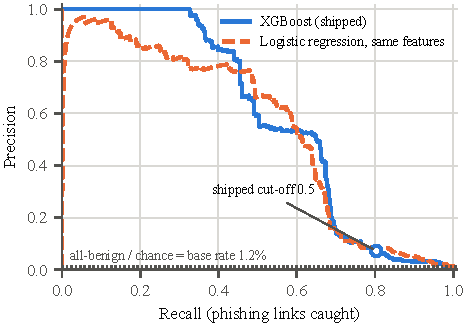
\includegraphics[width=\columnwidth]{figs/url_pr.pdf}
\caption{Precision--recall on 50,600 live links (OpenPhish vs Tranco). Both learners
see the same 15 host-name features.}
\label{fig:url}
\end{figure}

\subsection{Attachments}
On 615 phishing mails that carry attachments, the share not cleared as SAFE rises from
93.0\% to 93.8\% [95\% CI 91.6, 95.5], and on 1,606 real mails with
attachments it adds no false alarms. The gain is small because the content
model already catches most of this mail. A QR-code check was built but is
switched off: the phishing corpus contains no QR codes, so its benefit could
not be measured.

\subsection{Fusion and the behaviour engine}
CEAS-08 is the only public corpus with ham, spam, real senders and dates, so
the behaviour engine is tested on its stream: profiles are built from 1--7
August and the 8 August mail is scored once. The content model's spam recall
is 0.611; once behaviour may escalate content-clean mail, it is 0.912. The cost
is 8.5\% of legitimate mail the content model had cleared now marked
SUSPICIOUS (never PHISHING). The gain is at this operating point only: as a
ranking, the weighted sum is \emph{worse} than content alone (AUC 0.963 vs
0.990), and a logistic-regression stacker trained on the first half of the test
day does not beat content on the second half (0.947 vs 0.974). Behaviour helps by
lifting mail that content has cleared, not by reordering mail in general. Almost all of the signal is first contact and new
domain. Four features (bursts, blasts, odd hours, style change) are
\emph{inverted} on CEAS (train-window AUC 0.18--0.32) because its recipients are
mailing lists; they carry no weight in the hand rule. An isolation
forest~\cite{lestari2025isolation} on the same features scores AUC 0.595 when
fitted on normal traffic and 0.221 when fitted on the whole stream, where half the
mail is spam and ``first contact'' is the majority pattern.

On Gmail, an SPF/DKIM/DMARC failure occurs in 35.8\% of phishing\_pot mail and
in 0.5--0.8\% of two personal mailboxes. The repeat-sender damp cut the third
person's false alarms from 4.6\% to 2.5\% without losing any phishing; it arms
on only about a third of legitimate mail, because most real mail links to some
other domain. The crowd-report layer is unmeasured: there is no multi-user log.

\subsection{Voice content}
Table~\ref{tab:voice} reports the content layer. The strongest result is on
real scam calls from seven YouTube channels never used in training (96.2\%,
Wilson CI [90.6, 98.5]) against two false alarms in 723 held-out bank calls
(0.3\%, [0.1, 1.0]). Two numbers are weak. FTC robocalls are caught only
24.5\% of the time; a robocall is the bait (``press 1''), and the
recording stops before the ask. On the 27 recorded two-party calls, the score is
the maximum over windows, so a 17-minute call gets about 500 chances to cross the
band and a short one gets seven; per-window separation is much weaker than the
call-level 81.5\% suggests.

\begin{table}[t]
\caption{Voice content layer on held-out calls}
\label{tab:voice}
\centering\footnotesize
\setlength{\tabcolsep}{3pt}
\begin{tabular}{@{}p{4.6cm}r@{}}
\toprule
Test set & Result \\
\midrule
Scam-baiting calls, 7 unseen channels ($n$=105), caught & 96.2\% \\
HarperValleyBank half B ($n$=723), false alarms & 0.3\% \\
27 two-party calls, accuracy / AUC & 81.5\% / 0.850 \\
Scam Dialogue (synthetic, $n$=1,598), accuracy / AUC & 86.4\% / 0.917 \\
FTC robocalls ($n$=1,353), caught (in-source for act model) & 24.5\% \\
\bottomrule
\end{tabular}
\end{table}

\subsection{Synthetic voice}
Fig.~\ref{fig:spoof} compares the shipped spoof head with the previous one
(ASVspoof 2019 + 5 only). On modern voices from 41 MLAAD synthesis tools and
Edge-TTS that neither head saw, passed through a phone channel, the shipped head
catches 85.8\% and 96.7\%; the previous head caught 20.0\% of each. It also
flags fewer real video-call voices (0.6\% vs 2.9\%). The price is visible in the
figure: equal error rate rises on the ASVspoof 2021 PSTN subset (6.5$\to$8.1\%, CI [6.3, 10.3])
and on ASVspoof 5 (9.5$\to$14.2\%, CI [13.6, 14.9]), and on 105 real scam calls from seven unseen
channels the new head flags 6.7\% as synthetic [3.3, 13.1] against 1.9\%
before. This \emph{failed} one of the rules fixed in advance; the model was
promoted by choice because unseen modern voices are the realistic threat, and
because the spoof slot can only raise risk, never decide a verdict alone.
On In-the-Wild deepfakes~\cite{muller2022itw}, a head trained on ASVspoof 2019
alone reaches 38.8\% EER; the shipped head reaches 13.3\% (clean) and 16.3\% (phone).

\begin{figure}[t]
\centering
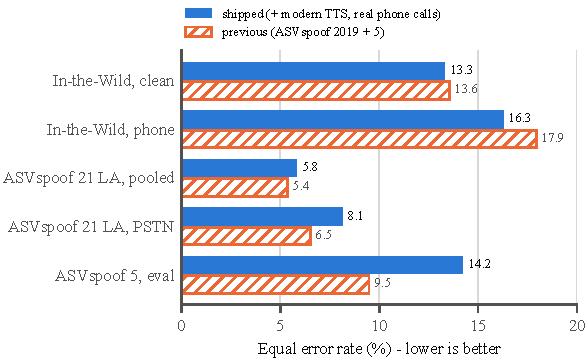
\includegraphics[width=\columnwidth]{figs/spoof_eer.pdf}
\caption{Spoof detection equal error rate. The shipped head was trained for unseen
modern voices and real phone audio, and is worse on the ASVspoof laboratory sets.}
\label{fig:spoof}
\end{figure}

\subsection{Persuasion head}\label{sec:persuasion}
On true phishing mail, the head fires (score $\ge 0.5$) for reward 51.5\%,
urgency 43.4\%, authority 36.5\%, fear 10.9\% and scarcity 10.8\% of mails.
These are firing rates, not accuracy: the labels come from regular
expressions, and no hand-labelled test set exists. We therefore use the head
only to word explanations, never to score.

\subsection{Explanation faithfulness}\label{sec:faith}
A deletion test checks that the explanations name the evidence the model used.
Deleting the three or so words the SMS explainer names drops $p$(smishing) by 0.280
(in-source) and 0.394 (held-out), against 0.030 and 0.040 for three random words;
the verdict flips 24.8\% and 46.7\% of the time versus 2.7\% and 4.8\%. Resetting the
three top TreeSHAP link features to the benign median drops the score by 0.378 and
flips 53.7\% of verdicts, against 0.066 and 9.1\% for random features.

\subsection{Cost}
Table~\ref{tab:cost} gives model sizes and single-message latency. The SMS and link models together take 2.1\,MB on the phone and score a message in a few milliseconds on a CPU. Whisper transcribes at 0.051$\times$ real time (3.1\,s per audio minute), so the voice path keeps up with a live call on one consumer GPU; the spoof head adds 36\,ms per 4\,s clip.

\begin{table}[t]
\caption{Size and median batch-1 latency (laptop, Section~III-C)}
\label{tab:cost}
\centering\footnotesize
\setlength{\tabcolsep}{2.5pt}
\begin{tabular}{@{}lrrl@{}}
\toprule
Component & Size & Disk & Latency \\
\midrule
SMS char 3--5 + LR & 0.19M wts & 2.6\,MB & 0.9\,ms CPU \\
URL XGBoost (400 trees) & 15 feat. & 2.0\,MB & 3.6\,ms CPU \\
Phone assets (SMS + URL) & --- & 2.1\,MB & on-device \\
Email DistilBERT + persuasion & 66M & 266\,MB & 15.0\,ms GPU \\
Voice act model (DistilBERT) & 67M & 269\,MB & 13.1\,ms GPU \\
Spoof: XLS-R 300M + LR head & 315M & 1.2\,GB$^\dagger$ & 36.2\,ms / 4\,s clip \\
Whisper small (fp16) & 244M & --- & 3.1\,s / audio min \\
\midrule
\multicolumn{4}{@{}l}{$^\dagger$ shared pretrained encoder; the trained head itself is 0.1\,MB.}\\
\bottomrule
\end{tabular}
\end{table}

% =====================================================================
\section{Corpus Artifacts}\label{sec:artifacts}

The most repeated finding of this project is that a high score often measured
the \emph{dataset}. Table~\ref{tab:artifacts} lists every case we found. Each one
gave a convincing number, and each was caught only by an ablation, an
outside test set, or by checking what a single feature scores alone. This is the
pitfall Arp et al.\ call spurious correlation~\cite{arp2022dos}; we add
measured, channel-specific instances of it.

\begin{table*}[t]
\caption{Corpus artifacts found in this project: what the feature really encoded, and what it cost}
\label{tab:artifacts}
\centering\footnotesize
\setlength{\tabcolsep}{4pt}
\begin{tabular}{@{}p{0.3cm}p{3.1cm}p{6.6cm}p{6.6cm}@{}}
\toprule
\# & Where & What the model learned & Measured effect \\
\midrule
1 & PhiUSIIL URLs & 100\% of legitimate URLs are HTTPS with no path & Scheme/path features: AUC 0.331 on live links (below chance) \\
2 & CEAS-08 has-URL flag & 2008 ham was link-heavy list digests; spam was plain text & Flag alone AUC 0.395; stacker shows false 0.986 \\
3 & CEAS-08 labels & Its ``phishing'' label means spam & Model catches 30.9\% of real (Nazario) phishing \\
4 & Email phishing source & Public phishing corpora share one style & Public-only model: 98.9\% own-source, 42.6\% on 2025--26 mail \\
5 & Enron vs modern ham & Era and mail software, not intent & Surface features split Enron from 2025 ham at AUC 0.885 \\
6 & Speech transcripts & Scam = ASR output; legitimate = typed text & In-source AUC 1.000; real calls 0.576 \\
7 & UCI SMS & UK currency and freephone numbers mark scams & Top smishing features ``\pounds1'', ``0800''; recall drop off-corpus \\
8 & Indian SMS spam class & No Indian marketing rows existed & Offer + link read as smishing; a real coupon scored 0.631 \\
9 & Indian SMS metadata & ``Platform found'' column (Call/Telegram = 100\% fraud) & A free label; column withheld \\
10 & Indian SMS templates & 3,200 rows from $\sim$1,400 templates & Random split gives TF-IDF F1 0.99; grouped split used \\
11 & Mishra--Soni releases & 10,191-row file is a rebalanced copy of the 5,971 one & Train/test leak unless deduplicated \\
12 & CEAS behaviour & Recipients are mailing lists & Burst/blast/hour features inverted (AUC 0.18--0.32) \\
13 & Spoof, clean training & Clean real speech vs clean fakes & Real voices through a phone line score 0.841 ``fake'' \\
\bottomrule
\end{tabular}
\end{table*}

\subsection{Error analysis}
\textit{SMS} errors on the held-out corpus are mostly smishing written in
another country's conventions (currency, short codes) that the UK-heavy training
mix has not seen. \textit{Email} false alarms on the unseen person are
concentrated in one newsletter sender (28 of its 358 mails), and spam is missed when it reads like a newsletter, which is a
consent problem, not a content one. \textit{Voice} misses are relational
scams with no transactional words (a ``relative in trouble'', romance or
investment-group openers), and a real police officer saying ``police'' is the
one remaining false alarm on our 50 authored test transcripts.

\subsection{Threats to validity}
(i) Two of three mailboxes and the SMS inbox belong to team members; the third
mailbox shaped the final email recipe, so it is not fully independent.
(ii) The held-out SMS corpus shares an origin with a training release; it is
deduplicated by exact text only. (iii) The scam-baiting victims are performers;
the act model scores only the caller's turns, but channel choice is ours.
(iv) The behaviour rules for SMS and calls are unmeasured, because no public
corpus has sender or caller fields. (v) Crowd reports are unmeasured. (vi) The
second attempt against the scam-baiting set weakens that test as evidence.

% =====================================================================
\section{Privacy, Ethics and Sustainability}\label{sec:ethics}
The design follows the data-minimisation duty of India's DPDP
Act~\cite{dpdp2023} by construction rather than by policy. The phone scores
SMS entirely on the device with exported copies of the models and holds no
Internet permission, so neither messages nor verdicts can leave it; an optional
inbox report is shared only by the user, with codes, amounts and account
numbers masked. The SMS model's vocabulary, stored in plain text on the phone,
is fitted on public corpora only, so no string from a private inbox ships. Gmail bodies are never stored:
the dashboard fetches a mail live when the user opens it, and stored scans keep
an attachment's file type, never its name. Safe Browsing receives only 4-byte
hash prefixes. Voice analysis runs on the server, not the phone, and only on audio
the user uploads. Private corpora are never published, and the weights trained on
them are not released.

Small models keep inference cheap (Table~\ref{tab:cost}): the SMS model
runs on a phone CPU, and no generative model runs at inference time. Reducing
fraud against first-time digital users supports SDG~8 and SDG~16.

% =====================================================================
\section{Limitations and Future Work}
Smishing recall off-corpus (0.786) is below target and needs regional data,
which is scarce: no public Indian scam-call corpus exists. Sender and caller
behaviour rules need a real deployment log to be measured, and the persuasion
head needs a hand-labelled set. The spoof head trades laboratory scores for
modern-voice coverage and still flags 6.7\% of real scam-call audio as
synthetic. The QR-code check awaits a fair evaluation set. Future work is a
federated update for the phone models and a multi-user study of crowd reports.

% =====================================================================
\section{Conclusion}
A three-channel scam detector can be small, explainable and private, but only
an evaluation that refuses random splits shows where it is weak. Sender
behaviour broke a content-only spam ceiling (0.611$\to$0.912 recall); content
models held up on later and unseen data for email (0.986 phishing recall,
temporal) and for scam calls (96.2\% on unseen channels), and degraded
honestly where the data shifted most (SMS, 0.786 smishing recall). The thirteen
artifacts in Table~\ref{tab:artifacts} are, in our view, the most transferable
lesson: each would have been a headline number.

\section*{Data and Code Availability}
Code, evaluation scripts and the measurement logs behind every number are in
the project repository (private while private-data weights are in it; to be
released with retrained public-only weights). Public datasets are cited where
used. Private mailboxes, the SMS inbox and models trained on them are not shared.

\bibliographystyle{IEEEtran}
\bibliography{refs}

\end{document}
